\documentclass{article}

\usepackage{graphicx}
\usepackage{tikz}
\usepackage{tikzsymbols}
\usetikzlibrary{calc,patterns,shapes.geometric}
\pagestyle{empty}
\usepackage[margin=0pt]{geometry}
\geometry{papersize={14in,12in}}

\def\centerarc[#1](#2)(#3:#4:#5){\draw[#1] ($(#2)+({#5*cos(#3)},{#5*sin(#3)})$) arc (#3:#4:#5);}

\begin{document}
	\begin{figure}
		\centering
		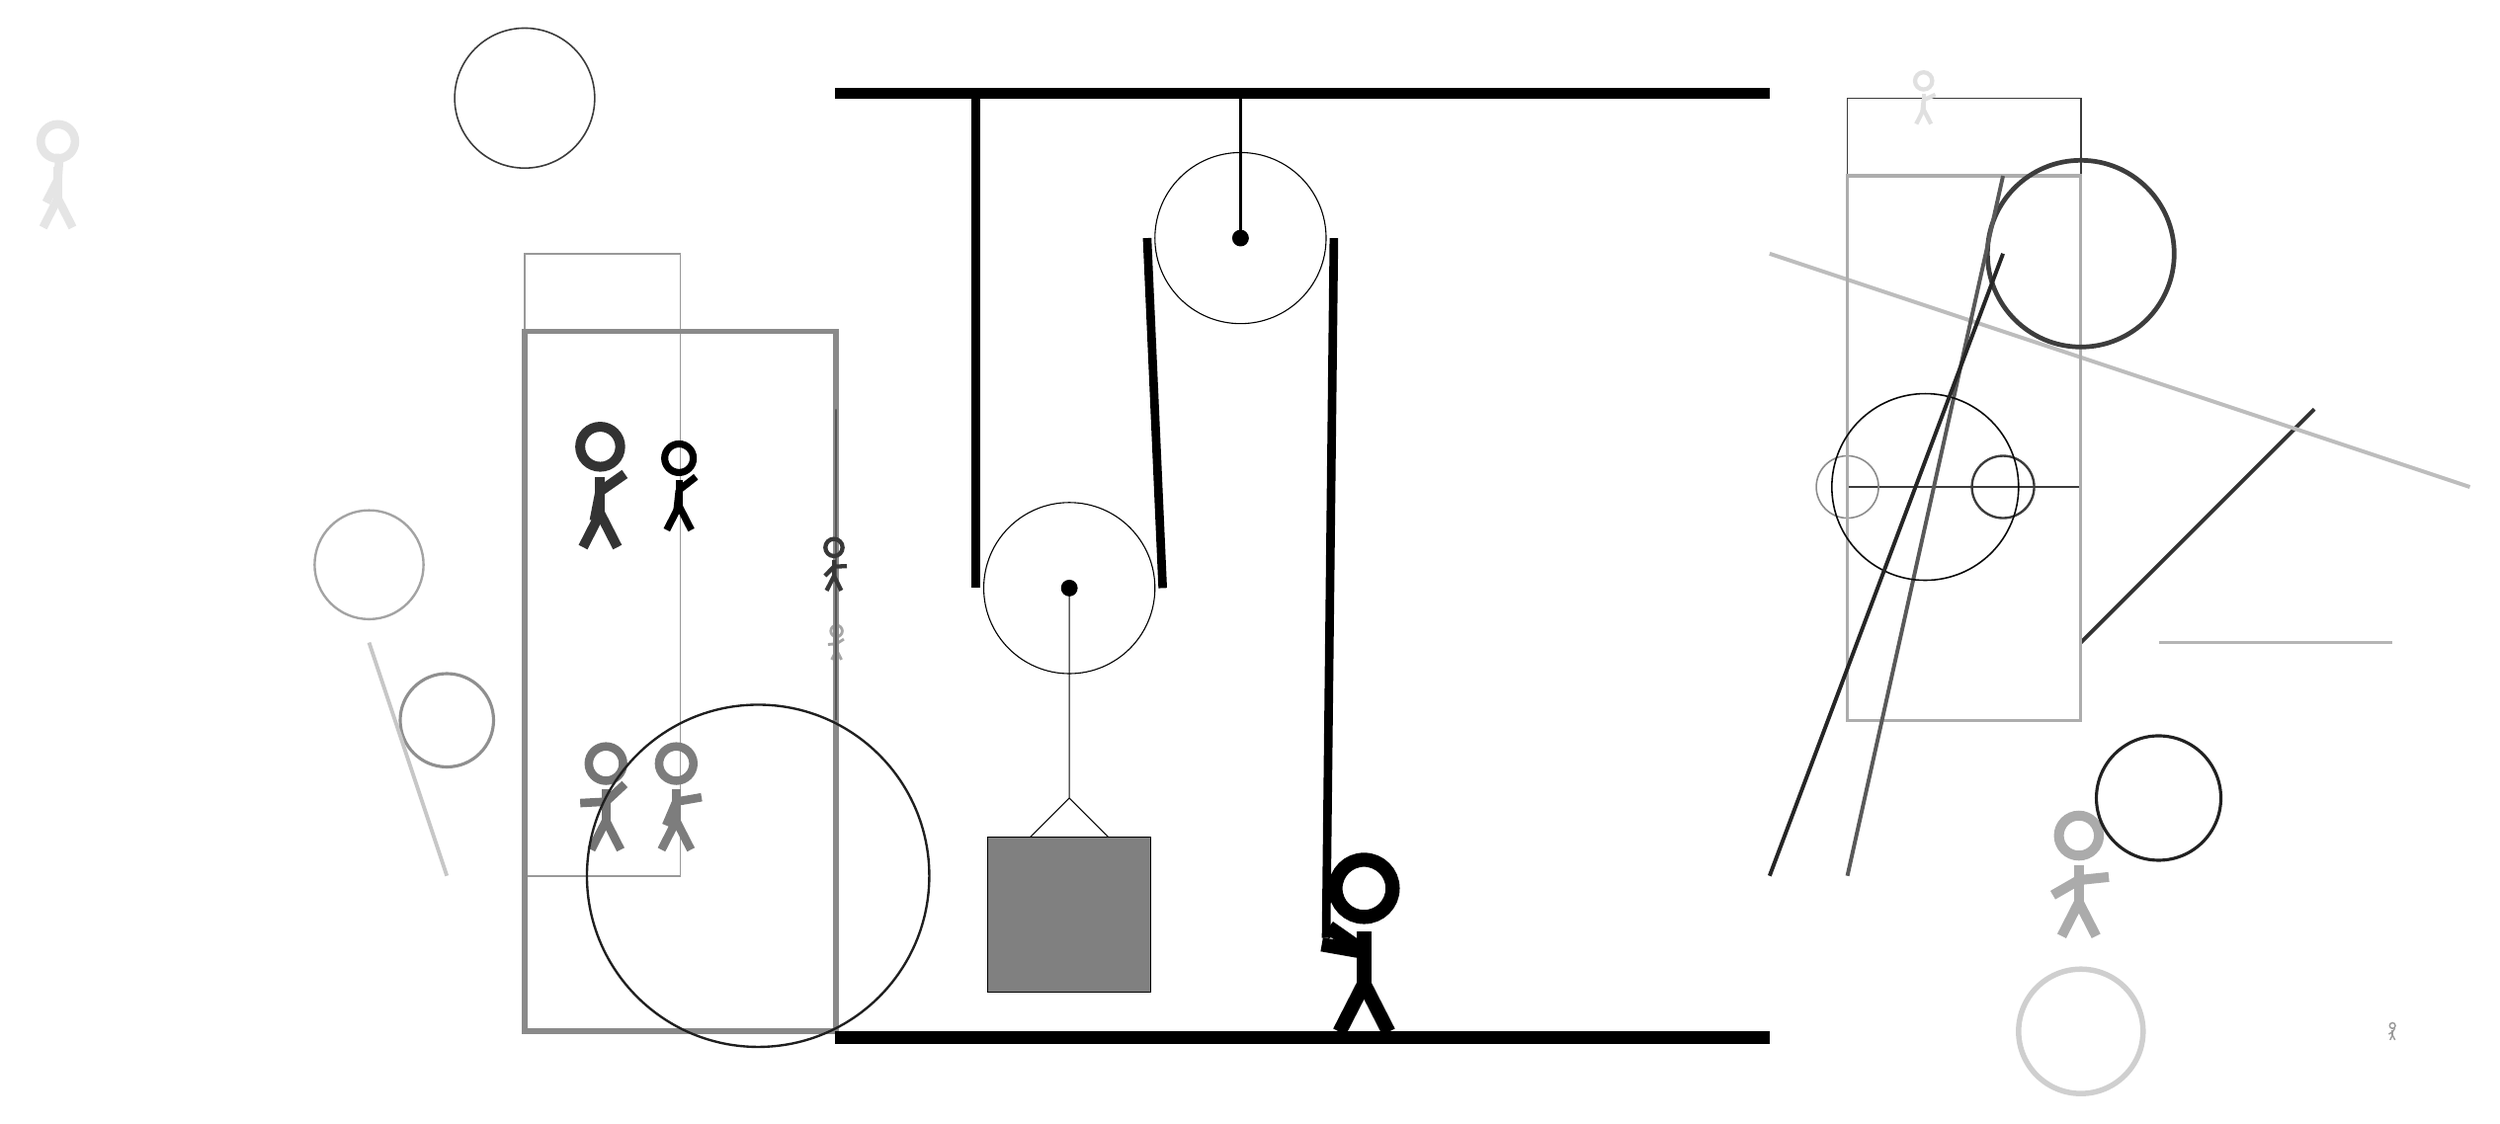
\begin{tikzpicture}
			%%%%% START %%%%%
			
			\draw[fill=black] (-2, 9) rectangle (10, 9.125);
			
			\draw [line width=0.4mm, color=black!44](-7, 1) circle (0.6);
			
			\draw[line width=0.2mm, color=black!40] (-4, 7) rectangle (-6, -1);
			\node[line width=0.2mm, color=black!33] at (14, -1) {\Strichmaxerl[7][30][6]};
			\draw [line width=0.4mm, color=black!87](15, 0) circle (0.8);
			\draw[line width=0.5mm, color=black!22](-7, -1) -- (-8, 2);
			
			\draw [line width=0.3mm, color=black!36](-8, 3) circle (0.7);
			\draw[line width=0.2mm, color=black!77] (11, 9) rectangle (14, 4);
			
			\node[line width=0.6mm, color=black!80] at (-5, 4) {\Strichmaxerl[7][79][35]};
			\draw[line width=0.5mm, color=black!80](14, 2) -- (17, 5);
			\draw[line width=0.5mm, color=black!26](10, 7) -- (19, 4);
			
			\node[line width=0.2mm, color=black!51] at (-4, 0) {\Strichmaxerl[6][67][10]};
			
			\node[line width=0.5mm, color=black!35] at (-2, 2) {\Strichmaxerl[2][5][32]};
			\draw [line width=0.2mm, color=black!45](11, 4) circle (0.4);
			
			\node[line width=0.3mm, color=black!10] at (-12, 8) {\Strichmaxerl[6][63][86]};
			\draw[line width=0.4mm, color=black!32] (11, 8) rectangle (14, 1);
			\draw [line width=0.6mm, color=black!76](14, 7) circle (1.2);
			\draw [line width=0.3mm, color=black!77](13, 4) circle (0.4);
			
			\node[line width=0.4mm, color=black!54] at (-5, 0) {\Strichmaxerl[6][3][43]};
			\draw[line width=0.5mm, color=black!65](11, -1) -- (13, 8);
			\draw[line width=0.5mm, color=black!29](15, 2) -- (18, 2);
			\node[line width=0.7mm, color=black!40] at (18, -3) {\Strichmaxerl[1][30][57]};
			
			\draw [line width=0.7mm, color=black!19](14, -3) circle (0.8);
			
			\node[line width=0.5mm, color=black!100] at (-4, 4) {\Strichmaxerl[5][84][38]};
			\draw[line width=0.7mm, color=black!46] (-2, -3) rectangle (-6, 6);
			\draw [line width=0.3mm, color=black!88](-3, -1) circle (2.2);
			\node[line width=0.3mm, color=black!12] at (12, 9) {\Strichmaxerl[3][84][24]};
			
			\draw [line width=0.2mm, color=black!97](12, 4) circle (1.2);
			\draw[line width=0.2mm, color=black!66] (-2, 5) rectangle (-2, 1);
			
			\node[line width=0.7mm, color=black!78] at (-2, 3) {\Strichmaxerl[3][46][2]};
			
			\draw [line width=0.2mm, color=black!77](-6, 9) circle (0.9);
			\draw[line width=0.5mm, color=black!85](10, -1) -- (13, 7);
			
			\draw (3.2, 7.2) circle (1.1);
			\draw[fill=black] (3.2, 7.2) circle (0.1);
			\draw[thick] (3.2, 7.2) -- (3.2, 9);
			
			\draw (1, 2.7) circle (1.1);
			\draw[fill=black] (1, 2.7) circle (0.1);
			
			\draw (1, 2.7) -- (1, 0) -- (0.5, -0.5);
			\draw (1, 0) -- (1.5, -0.5);
			\draw[fill=black!50] (-0.05, -0.5) rectangle (2.05, -2.5);
			
			\draw[line width=1.1mm] (-0.2, 9) -- (-0.2, 2.7);
			\centerarc[line width=1.1mm](1, 2.7)(180:360:1.2000000000000002);
			\draw[line width=1.1mm](2.2, 2.7) -- (2.0, 7.2);
			\centerarc[line width=1.1mm](3.2, 7.2)(0:180:1.2000000000000002);
			\draw[line width=1.1mm](4.4, 7.2) -- (4.3, -1.8);
			
			\node at (4.7, -1.9) {\Strichmaxerl[10][-35][170]};
			
			\draw[fill=black] (-2, -3) rectangle (10, -3.15);
			
			%%%%% END %%%%%
		\end{tikzpicture}
	\end{figure}	
\end{document}